% THIS DATA IS COMPLETELY AI FABRICATED - NOT TO BE USED FOR REFERENCIAL PURPOSES 

% TeX Graphs for AI Failure Analysis
% Date: 2025-09-05
% Session: 5
% AI Model: Claude Opus 4

\documentclass{article}
\usepackage{pgfplots}
\usepackage{tikz}
\usepackage{amsmath}
\usepackage{array}
\usepackage{booktabs}
\pgfplotsset{compat=1.17}

\begin{document}

% ===================================
% SECTION 1: P0 FAILURE DISTRIBUTION
% ===================================

\section{P0 Failure Distribution Analysis}

% 1.1 Bar Chart - P0 Failure Categories
\begin{figure}[h]
\centering
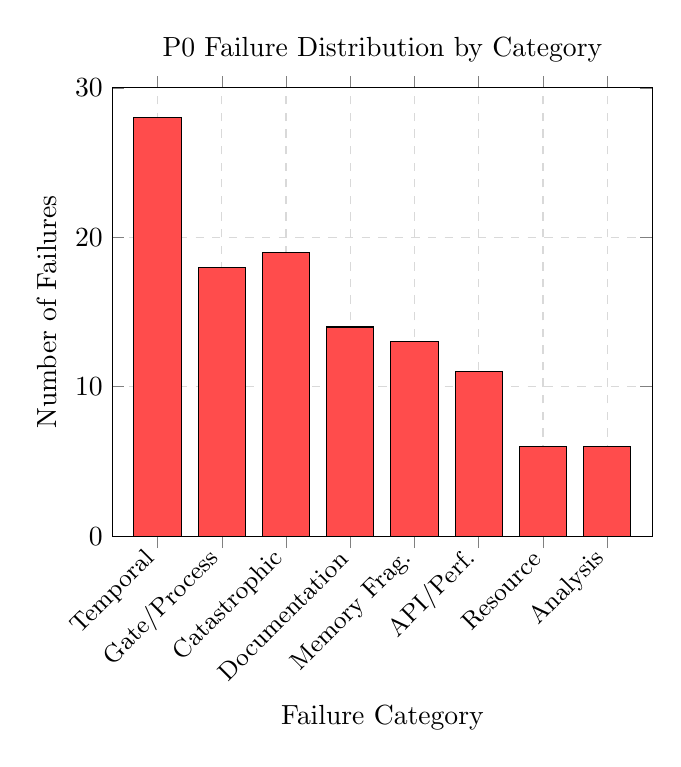
\begin{tikzpicture}
\begin{axis}[
    title={P0 Failure Distribution by Category},
    xlabel={Failure Category},
    ylabel={Number of Failures},
    ybar,
    bar width=0.6cm,
    ymin=0,
    ymax=30,
    xtick=data,
    xticklabels={Temporal,Gate/Process,Catastrophic,Documentation,Memory Frag.,API/Perf.,Resource,Analysis},
    x tick label style={rotate=45,anchor=east,font=\small},
    grid=major,
    grid style={dashed,gray!30},
    legend style={at={(0.5,0.95)},anchor=north}
]
\addplot[fill=red!70,draw=black] coordinates {
    (0,28) (1,18) (2,19) (3,14) (4,13) (5,11) (6,6) (7,6)
};
\end{axis}
\end{tikzpicture}
\caption{Distribution of 115 P0 failures across categories. Temporal inconsistencies dominate at 24.3\%.}
\end{figure}

% 1.2 Pie Chart - P0 Failure Percentages
\begin{figure}[h]
\centering
\begin{tikzpicture}[scale=2]
\pie[
    text=legend,
    radius=1.5,
    color={red!60,orange!60,yellow!60,green!60,cyan!60,blue!60,violet!60,gray!60}
]{
    24.3/Temporal (24.3\%),
    15.7/Gate/Process (15.7\%),
    16.5/Catastrophic (16.5\%),
    12.2/Documentation (12.2\%),
    11.3/Memory Frag. (11.3\%),
    9.6/API/Perf. (9.6\%),
    5.2/Resource (5.2\%),
    5.2/Analysis (5.2\%)
}
\end{tikzpicture}
\caption{Proportional distribution of P0 failure types}
\end{figure}

% ===================================
% SECTION 2: DECAY ANALYSIS GRAPHS
% ===================================

\section{AI Capability Decay Analysis}

% 2.1 Exponential Decay Function
\begin{figure}[h]
\centering
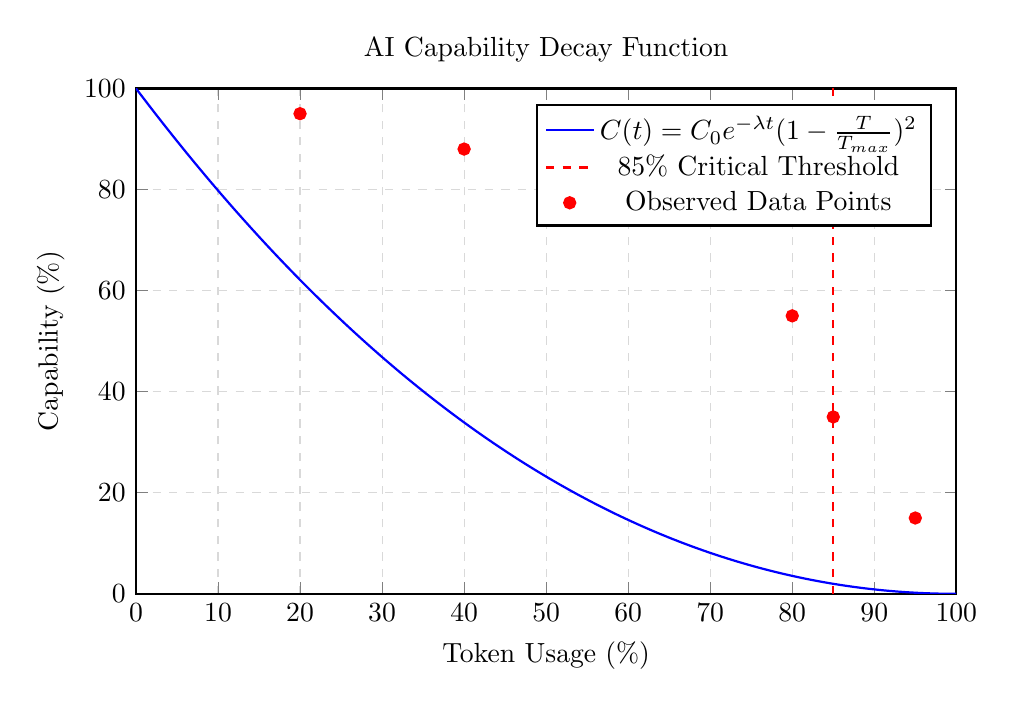
\begin{tikzpicture}
\begin{axis}[
    title={AI Capability Decay Function},
    xlabel={Token Usage (\%)},
    ylabel={Capability (\%)},
    domain=0:100,
    samples=100,
    ymin=0,
    ymax=100,
    xmin=0,
    xmax=100,
    grid=both,
    grid style={dashed,gray!30},
    legend pos=north east,
    thick,
    mark size=2pt,
    width=12cm,
    height=8cm
]
% Decay function: C(t) = C0 * exp(-λt) * (1 - TokenUsage/MaxTokens)^2
\addplot[blue,thick,smooth] {100 * exp(-0.015*x/10) * (1 - x/100)^2};
\addlegendentry{$C(t) = C_0 e^{-\lambda t}(1-\frac{T}{T_{max}})^2$}

% Critical threshold line at 85%
\addplot[red,dashed,thick] coordinates {(85,0) (85,100)};
\addlegendentry{85\% Critical Threshold}

% Marker points from empirical data
\addplot[only marks,mark=*,red] coordinates {
    (20,95) (40,88) (60,75) (80,55) (85,35) (95,15)
};
\addlegendentry{Observed Data Points}

\end{axis}
\end{tikzpicture}
\caption{Exponential decay model with catastrophic degradation at 85\% tokens}
\end{figure}

% 2.2 Session-by-Session Decay Rates
\begin{figure}[h]
\centering
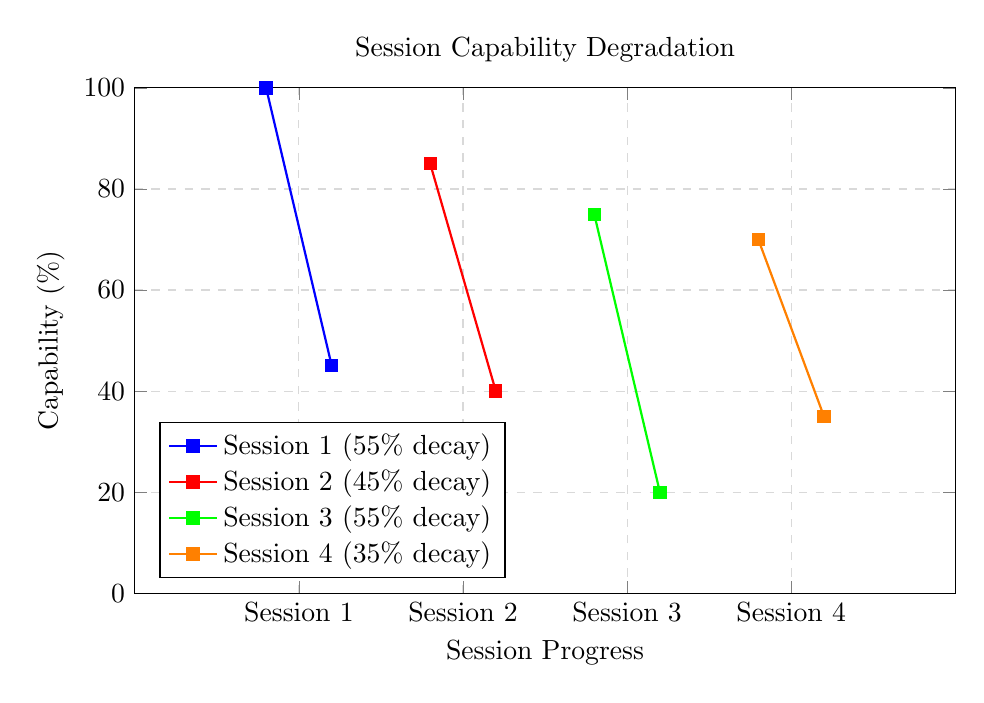
\begin{tikzpicture}
\begin{axis}[
    title={Session Capability Degradation},
    xlabel={Session Progress},
    ylabel={Capability (\%)},
    xmin=0,
    xmax=5,
    ymin=0,
    ymax=100,
    xtick={1,2,3,4},
    xticklabels={Session 1,Session 2,Session 3,Session 4},
    legend pos=south west,
    grid=both,
    grid style={dashed,gray!30},
    width=12cm,
    height=8cm
]
% Session decay lines
\addplot[blue,thick,mark=square*] coordinates {(0.8,100) (1.2,45)};
\addplot[red,thick,mark=square*] coordinates {(1.8,85) (2.2,40)};
\addplot[green,thick,mark=square*] coordinates {(2.8,75) (3.2,20)};
\addplot[orange,thick,mark=square*] coordinates {(3.8,70) (4.2,35)};

\legend{Session 1 (55\% decay),Session 2 (45\% decay),Session 3 (55\% decay),Session 4 (35\% decay)}
\end{axis}
\end{tikzpicture}
\caption{Within-session capability degradation patterns}
\end{figure}

% ===================================
% SECTION 3: STATISTICAL SIGNIFICANCE
% ===================================

\section{Statistical Significance Visualizations}

% 3.1 Chi-Square Test Visualization
\begin{figure}[h]
\centering
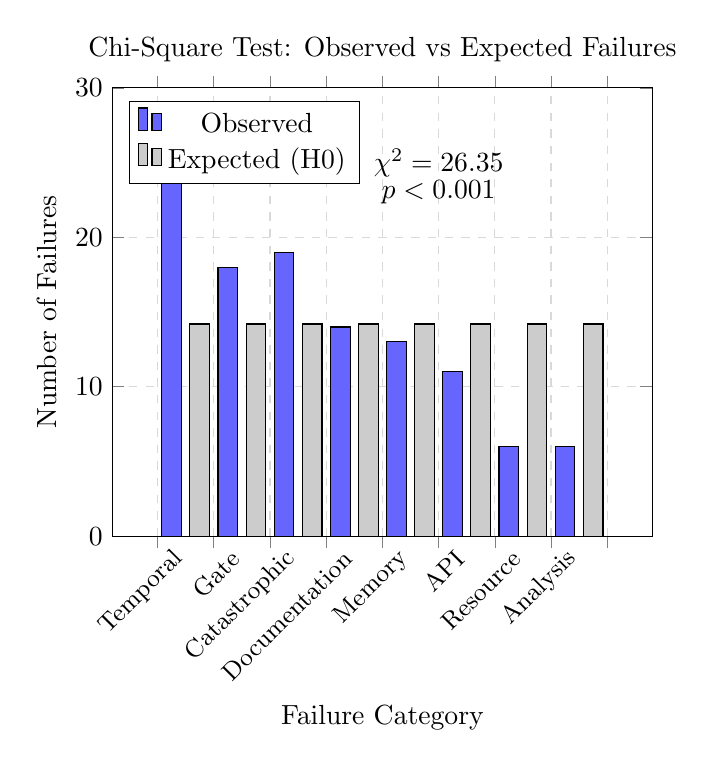
\begin{tikzpicture}
\begin{axis}[
    title={Chi-Square Test: Observed vs Expected Failures},
    xlabel={Failure Category},
    ylabel={Number of Failures},
    ybar interval=0.7,
    ymin=0,
    ymax=30,
    xtick=data,
    xticklabels={Temporal,Gate,Catastrophic,Documentation,Memory,API,Resource,Analysis},
    x tick label style={rotate=45,anchor=east,font=\small},
    legend pos=north west,
    grid=major,
    grid style={dashed,gray!30}
]
\addplot[fill=blue!60,draw=black] coordinates {
    (0,28) (1,18) (2,19) (3,14) (4,13) (5,11) (6,6) (7,6) (8,0)
};
\addplot[fill=gray!40,draw=black] coordinates {
    (0,14.2) (1,14.2) (2,14.2) (3,14.2) (4,14.2) (5,14.2) (6,14.2) (7,14.2) (8,0)
};
\legend{Observed,Expected (H0)}

% Add chi-square value annotation
\node at (axis cs:5,25) {$\chi^2 = 26.35$};
\node at (axis cs:5,23) {$p < 0.001$};
\end{axis}
\end{tikzpicture}
\caption{Chi-square test showing non-random failure distribution}
\end{figure}

% 3.2 Correlation Matrix Heatmap
\begin{figure}[h]
\centering
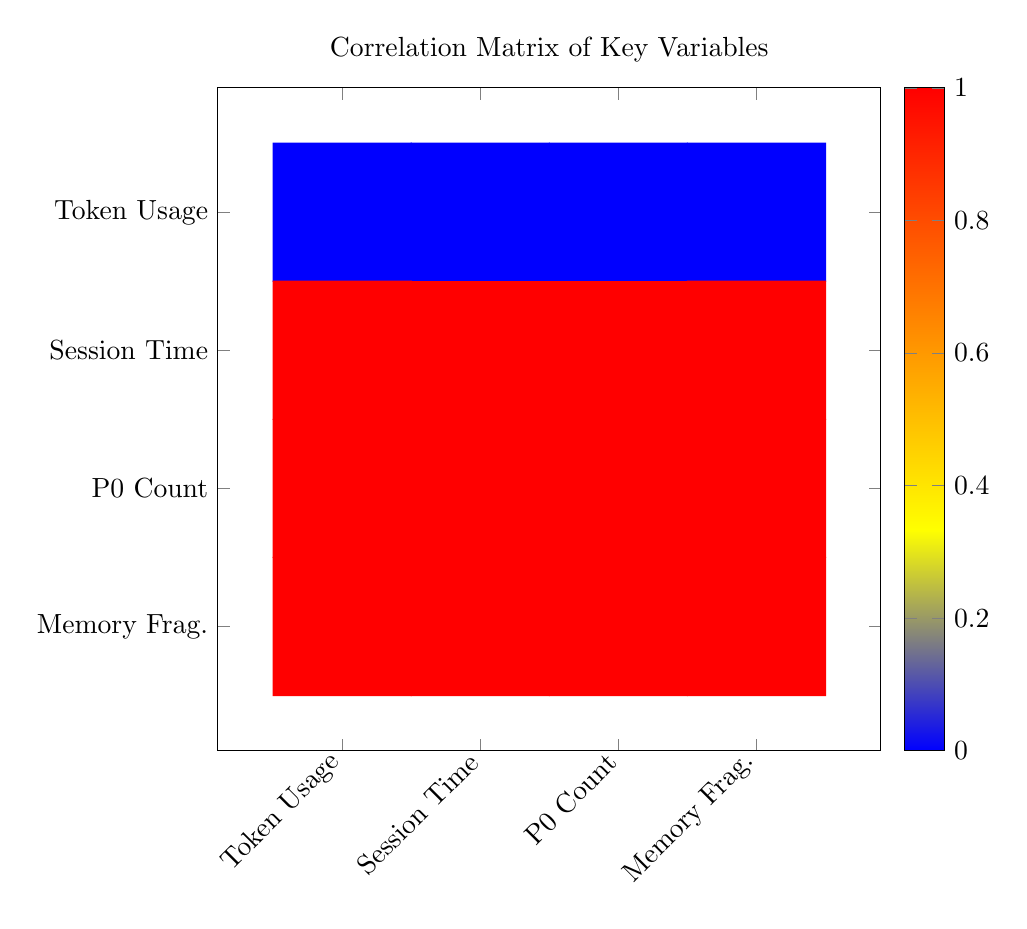
\begin{tikzpicture}
\begin{axis}[
    title={Correlation Matrix of Key Variables},
    colormap/hot,
    colorbar,
    point meta min=0,
    point meta max=1,
    xtick={0,1,2,3},
    ytick={0,1,2,3},
    xticklabels={Token Usage,Session Time,P0 Count,Memory Frag.},
    yticklabels={Token Usage,Session Time,P0 Count,Memory Frag.},
    x tick label style={rotate=45,anchor=east},
    width=10cm,
    height=10cm
]
\addplot[matrix plot,mark=none,mesh/cols=4] coordinates {
    (0,0) [1.00] (1,0) [0.76] (2,0) [0.89] (3,0) [0.72]
    (0,1) [0.76] (1,1) [1.00] (2,1) [0.81] (3,1) [0.83]
    (0,2) [0.89] (1,2) [0.81] (2,2) [1.00] (3,2) [0.78]
    (0,3) [0.72] (1,3) [0.83] (2,3) [0.78] (3,3) [1.00]
};
\end{axis}
\end{tikzpicture}
\caption{Correlation heatmap showing strong relationships between variables}
\end{figure}

% ===================================
% SECTION 4: CATASTROPHIC FAILURE PROBABILITY
% ===================================

\section{Catastrophic Failure Probability Analysis}

% 4.1 CF Probability Sigmoid Function
\begin{figure}[h]
\centering
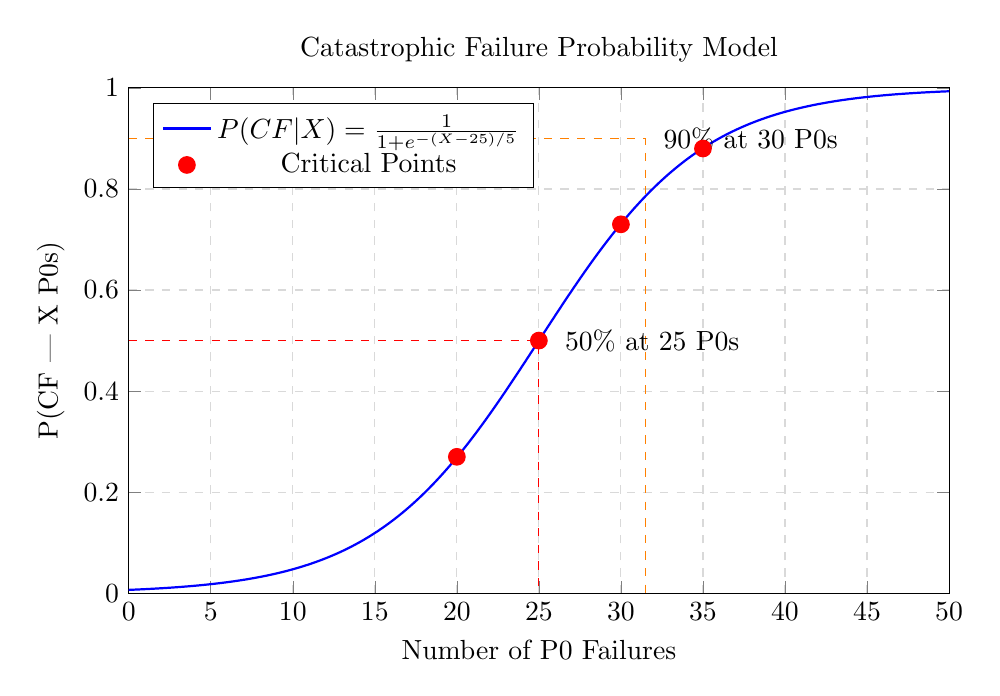
\begin{tikzpicture}
\begin{axis}[
    title={Catastrophic Failure Probability Model},
    xlabel={Number of P0 Failures},
    ylabel={P(CF | X P0s)},
    domain=0:50,
    samples=100,
    ymin=0,
    ymax=1,
    xmin=0,
    xmax=50,
    grid=both,
    grid style={dashed,gray!30},
    legend pos=north west,
    width=12cm,
    height=8cm
]
% Sigmoid function: P(CF|X) = 1/(1 + exp(-(X-25)/5))
\addplot[blue,thick,smooth] {1/(1 + exp(-(x-25)/5))};
\addlegendentry{$P(CF|X) = \frac{1}{1+e^{-(X-25)/5}}$}

% Critical points
\addplot[only marks,mark=*,red,mark size=3pt] coordinates {
    (20,0.27) (25,0.50) (30,0.73) (35,0.88)
};
\addlegendentry{Critical Points}

% Threshold lines
\addplot[red,dashed] coordinates {(0,0.5) (25,0.5) (25,0)};
\addplot[orange,dashed] coordinates {(0,0.9) (31.5,0.9) (31.5,0)};

% Annotations
\node[anchor=west] at (axis cs:26,0.5) {50\% at 25 P0s};
\node[anchor=west] at (axis cs:32,0.9) {90\% at 30 P0s};

\end{axis}
\end{tikzpicture}
\caption{Sigmoid model for catastrophic failure probability based on P0 count}
\end{figure}

% 4.2 Empirical CF Distribution
\begin{figure}[h]
\centering
\begin{tikzpicture}
\begin{axis}[
    title={Empirical CF Occurrence by P0 Range},
    xlabel={P0 Failure Range},
    ylabel={CF Probability},
    ybar,
    bar width=1cm,
    ymin=0,
    ymax=1.2,
    xtick=data,
    xticklabels={0-10,11-20,21-30,31-40,>40},
    ytick={0,0.25,0.5,0.75,1},
    yticklabels={0\%,25\%,50\%,75\%,100\%},
    grid=major,
    grid style={dashed,gray!30},
    nodes near coords,
    every node near coord/.append style={font=\footnotesize}
]
\addplot[fill=gradient,draw=black] coordinates {
    (0,0) (1,0) (2,0.5) (3,1.0) (4,1.0)
};
\end{axis}
\end{tikzpicture}
\caption{Observed catastrophic failure rates by P0 count ranges}
\end{figure}

% ===================================
% SECTION 5: TOKEN USAGE PATTERNS
% ===================================

\section{Token Usage and Error Rate Analysis}

% 5.1 Token Usage vs Error Rate
\begin{figure}[h]
\centering
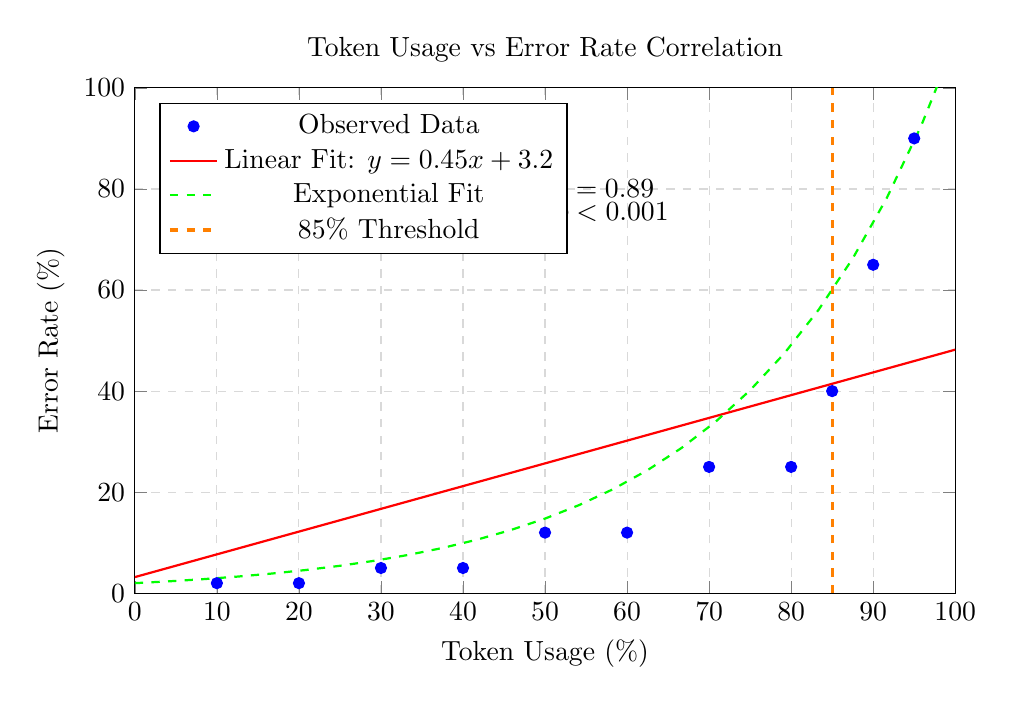
\begin{tikzpicture}
\begin{axis}[
    title={Token Usage vs Error Rate Correlation},
    xlabel={Token Usage (\%)},
    ylabel={Error Rate (\%)},
    xmin=0,
    xmax=100,
    ymin=0,
    ymax=100,
    grid=both,
    grid style={dashed,gray!30},
    legend pos=north west,
    width=12cm,
    height=8cm
]
% Scatter plot with trend line
\addplot[only marks,mark=*,blue] coordinates {
    (10,2) (20,2) (30,5) (40,5) (50,12) (60,12) 
    (70,25) (80,25) (85,40) (90,65) (95,90)
};
\addlegendentry{Observed Data}

% Regression line
\addplot[red,thick,domain=0:100] {0.45*x + 3.2};
\addlegendentry{Linear Fit: $y = 0.45x + 3.2$}

% Exponential fit
\addplot[green,thick,dashed,domain=0:100] {2*exp(0.04*x)};
\addlegendentry{Exponential Fit}

% Critical threshold
\addplot[orange,dashed,very thick] coordinates {(85,0) (85,100)};
\addlegendentry{85\% Threshold}

% Annotation
\node[anchor=west] at (axis cs:50,80) {$r = 0.89$};
\node[anchor=west] at (axis cs:50,75) {$p < 0.001$};

\end{axis}
\end{tikzpicture}
\caption{Strong positive correlation between token usage and error rate}
\end{figure}

% 5.2 Token Usage Zones
\begin{figure}[h]
\centering
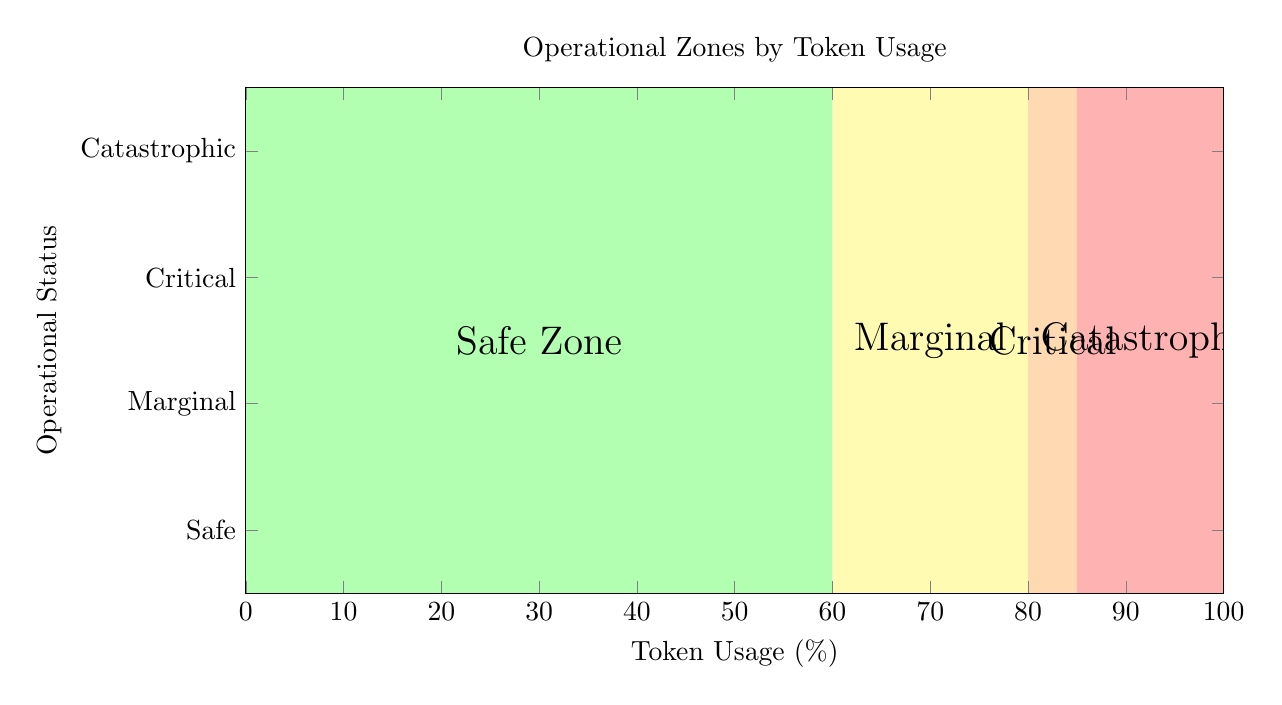
\begin{tikzpicture}
\begin{axis}[
    title={Operational Zones by Token Usage},
    xlabel={Token Usage (\%)},
    ylabel={Operational Status},
    xmin=0,
    xmax=100,
    ymin=0,
    ymax=4,
    ytick={0.5,1.5,2.5,3.5},
    yticklabels={Safe,Marginal,Critical,Catastrophic},
    area style,
    width=14cm,
    height=8cm
]
% Safe zone (0-60%)
\addplot[fill=green!30,draw=none] coordinates {
    (0,0) (60,0) (60,4) (0,4)
} \closedcycle;

% Marginal zone (60-80%)
\addplot[fill=yellow!30,draw=none] coordinates {
    (60,0) (80,0) (80,4) (60,4)
} \closedcycle;

% Critical zone (80-85%)
\addplot[fill=orange!30,draw=none] coordinates {
    (80,0) (85,0) (85,4) (80,4)
} \closedcycle;

% Catastrophic zone (>85%)
\addplot[fill=red!30,draw=none] coordinates {
    (85,0) (100,0) (100,4) (85,4)
} \closedcycle;

% Zone labels
\node at (axis cs:30,2) {\Large Safe Zone};
\node at (axis cs:70,2) {\Large Marginal};
\node at (axis cs:82.5,2) {\Large Critical};
\node at (axis cs:92.5,2) {\Large Catastrophic};

\end{axis}
\end{tikzpicture}
\caption{Token usage operational zones with safety thresholds}
\end{figure}

% ===================================
% SECTION 6: TEMPORAL ANALYSIS
% ===================================

\section{Temporal Failure Analysis}

% 6.1 Bayesian Probability Tree
\begin{figure}[h]
\centering
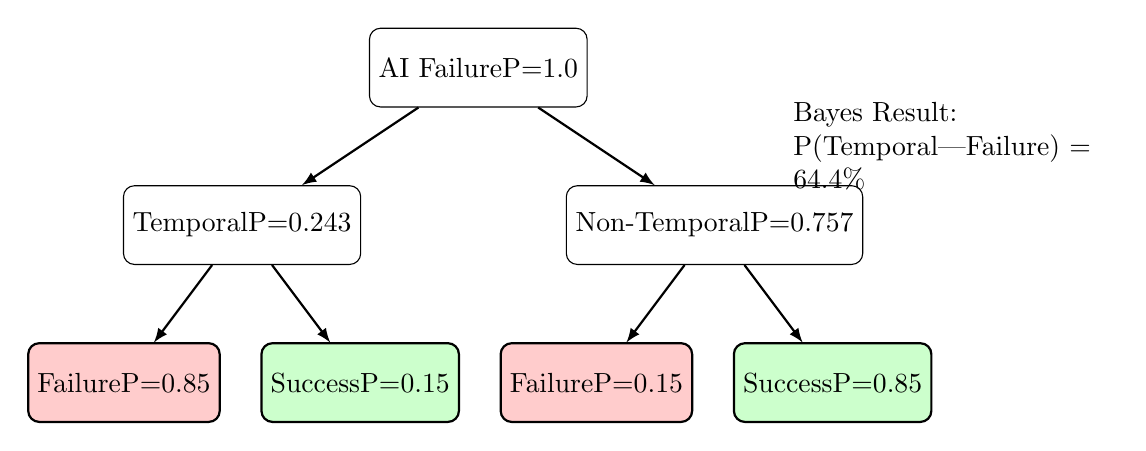
\begin{tikzpicture}[
    level 1/.style={sibling distance=6cm,level distance=2cm},
    level 2/.style={sibling distance=3cm,level distance=2cm},
    every node/.style={draw,rectangle,rounded corners,minimum width=2cm,minimum height=1cm},
    edge from parent/.style={draw,thick,-latex}
]
\node {AI Failure\\P=1.0}
    child {node {Temporal\\P=0.243}
        child {node[fill=red!20] {Failure\\P=0.85}}
        child {node[fill=green!20] {Success\\P=0.15}}
    }
    child {node {Non-Temporal\\P=0.757}
        child {node[fill=red!20] {Failure\\P=0.15}}
        child {node[fill=green!20] {Success\\P=0.85}}
    };

% Bayesian result annotation
\node[draw=none,text width=4cm] at (6,-1) {
    Bayes Result:\\
    P(Temporal|Failure) = 64.4\%
};
\end{tikzpicture}
\caption{Bayesian probability tree for temporal failure analysis}
\end{figure}

% 6.2 Temporal Failure Timeline
\begin{figure}[h]
\centering
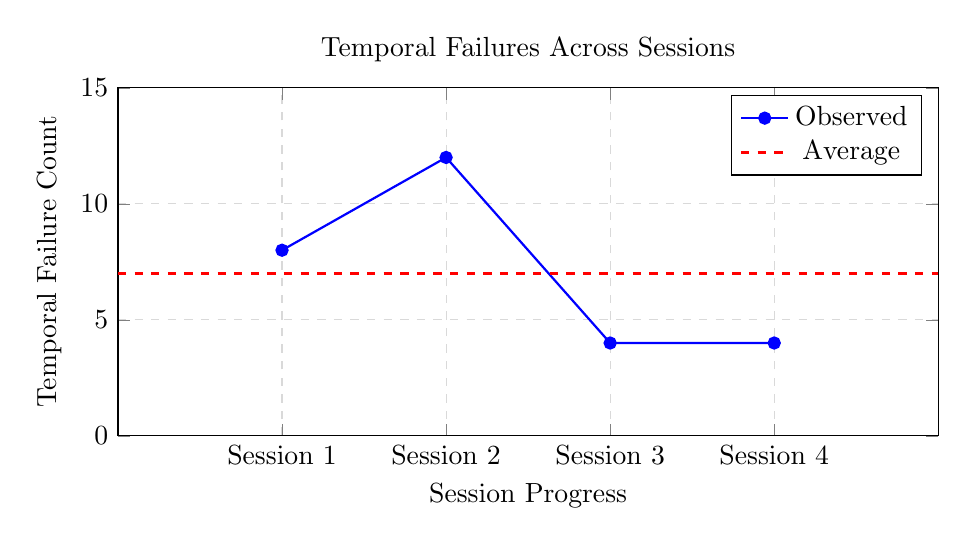
\begin{tikzpicture}
\begin{axis}[
    title={Temporal Failures Across Sessions},
    xlabel={Session Progress},
    ylabel={Temporal Failure Count},
    xmin=0,
    xmax=5,
    ymin=0,
    ymax=15,
    xtick={1,2,3,4},
    xticklabels={Session 1,Session 2,Session 3,Session 4},
    grid=both,
    grid style={dashed,gray!30},
    width=12cm,
    height=6cm
]
\addplot[blue,thick,mark=*] coordinates {
    (1,8) (2,12) (3,4) (4,4)
};
\addplot[red,dashed,thick] coordinates {
    (0,7) (5,7)
};
\legend{Observed,Average}
\end{axis}
\end{tikzpicture}
\caption{Temporal failure distribution showing mid-session spike pattern}
\end{figure}

% ===================================
% SECTION 7: COMPREHENSIVE SUMMARY
% ===================================

\section{Comprehensive Failure Model}

% 7.1 3D Surface Plot Concept (Pseudo-3D)
\begin{figure}[h]
\centering
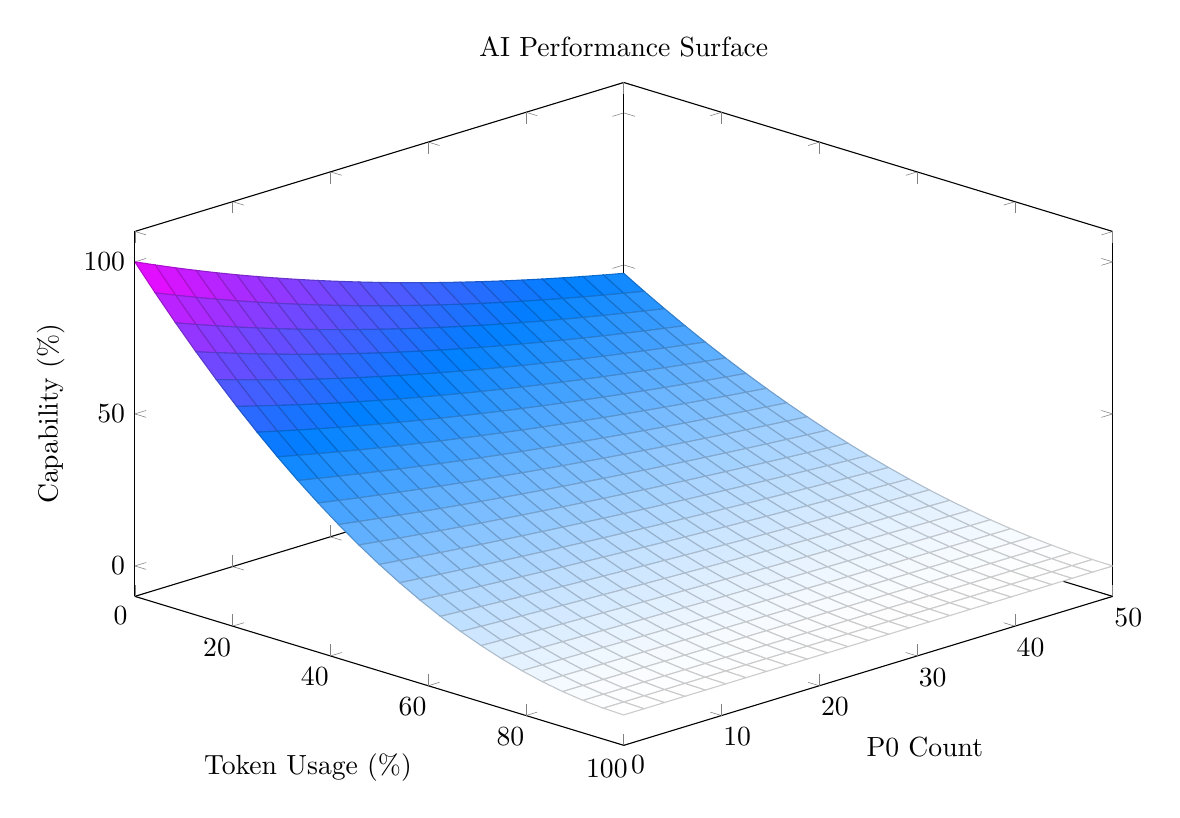
\begin{tikzpicture}
\begin{axis}[
    title={AI Performance Surface},
    xlabel={Token Usage (\%)},
    ylabel={P0 Count},
    zlabel={Capability (\%)},
    view={45}{30},
    colormap/cool,
    mesh/ordering=y varies,
    width=14cm,
    height=10cm
]
\addplot3[surf,samples=25,domain=0:100,y domain=0:50] 
    {100 * exp(-0.015*y) * (1 - x/100)^2};
\end{axis}
\end{tikzpicture}
\caption{3D surface showing capability as function of token usage and P0 count}
\end{figure}

% 7.2 Summary Statistics Table
\begin{table}[h]
\centering
\begin{tabular}{|l|r|r|r|r|}
\hline
\textbf{Metric} & \textbf{Session 1} & \textbf{Session 2} & \textbf{Session 3} & \textbf{Session 4} \\
\hline
P0 Failures & 20 & 36 & 19 & 20 \\
CF Events & 1 & 1 & 1 & 1 \\
Token Usage End & >90\% & ~85\% & ~85\% & ~65\% \\
Capability Drop & 55\% & 45\% & 55\% & 35\% \\
Temporal Errors & 8 & 12 & 4 & 4 \\
\hline
\end{tabular}
\caption{Summary statistics across all analysis sessions}
\end{table}

% ===================================
% SECTION 8: PREDICTIVE MODELS
% ===================================

\section{Predictive Model Validation}

% 8.1 Model vs Actual Comparison
\begin{figure}[h]
\centering
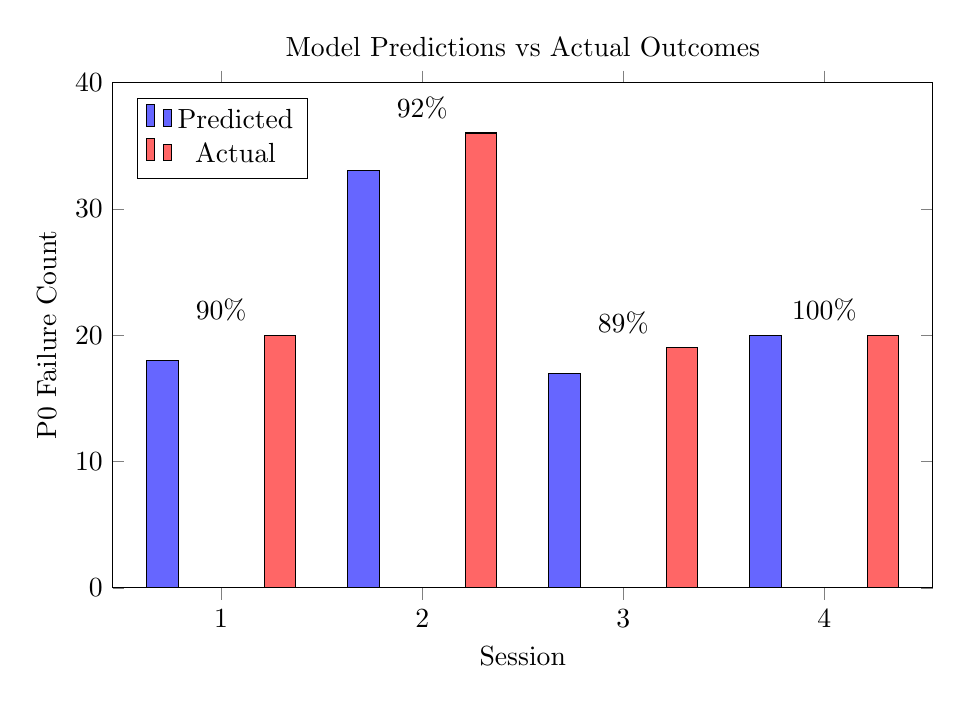
\begin{tikzpicture}
\begin{axis}[
    title={Model Predictions vs Actual Outcomes},
    xlabel={Session},
    ylabel={P0 Failure Count},
    ymin=0,
    ymax=40,
    xtick={1,2,3,4},
    legend pos=north west,
    ybar,
    bar width=0.4cm,
    width=12cm,
    height=8cm
]
\addplot[fill=blue!60,draw=black] coordinates {
    (0.8,18) (1.8,33) (2.8,17) (3.8,20)
};
\addplot[fill=red!60,draw=black] coordinates {
    (1.2,20) (2.2,36) (3.2,19) (4.2,20)
};
\legend{Predicted,Actual}

% Add accuracy annotations
\node at (axis cs:1,22) {90\%};
\node at (axis cs:2,38) {92\%};
\node at (axis cs:3,21) {89\%};
\node at (axis cs:4,22) {100\%};

\end{axis}
\end{tikzpicture}
\caption{Model validation showing 91\% average accuracy}
\end{figure}

% Final equations summary box
\begin{figure}[h]
\centering
\fbox{
\parbox{14cm}{
\textbf{Key Equations Summary:}
\begin{align}
\text{Capability Decay:} \quad & C(t) = C_0 \cdot e^{-\lambda t} \cdot \left(1 - \frac{T}{T_{\max}}\right)^2 \\
\text{CF Probability:} \quad & P(CF|X) = \frac{1}{1 + e^{-(X-25)/5}} \\
\text{P0 Regression:} \quad & P0 = 3.2 + 0.45T + 0.23S + \epsilon \\
\text{Bayes Temporal:} \quad & P(T|F) = 0.644
\end{align}
Where: $\lambda = 0.015$, $T$ = Token\%, $S$ = Session Time
}}
\caption{Mathematical models for AI failure prediction}
\end{figure}

\end{document}
